\documentclass{article}

\usepackage{fancyhdr}
\usepackage{hyperref} 
\usepackage{geometry} 
\geometry{a4paper, margin=1in}
\usepackage{graphicx}

\title{Computer Workshop \\ Final Homework}
\author{Hamidreza Yadegari}
\date{winter of 4031}

\hypersetup{hidelinks}
\pagestyle{fancy}
\fancyhead[L]{\thepage}

\begin{document}

\maketitle 
\thispagestyle{empty}
\newpage

\tableofcontents
\fancyhead[R]{Final HomeWork}
\setcounter{page}{1}
\newpage

\section{Git and GitHub}
    \subsection{Repository Initialization and Commits}
        First, we create a repository in GitHub by entering the desired name in its creation and ticking the box to create a `README` file. Then, using the command `git clone <repository-SSH-link>`, we transfer the above repository to our system. After that, we create a file called `main.tex` to write the answers to the questions. 

        Next, we use the command `git add .` to add it to the staging area. Then, we commit the file with the command:
        \begin{verbatim}
            git commit -m "add main.tex"
        \end{verbatim}
            Finally, we apply the changes to GitHub with the command:
        \begin{verbatim}
            git push origin master
        \end{verbatim}
        Now the project is ready for the next stage.
    \\
    \subsection{GitHub Actions for LaTeX Compilation}
        To set up GitHub Actions for LaTeX compilation, we first create a directory named `.github` in the main directory of the remote repository. Inside `.github`, we create another directory named `workflows`. Then, we create a file called `latex-build.yml` inside the `workflows` directory and add the settings from the site:
        \url{https://mrturkmen.com/posts/build-release-latex/}.
        
        In the `root\_file`, `asset\_path`, and `asset\_name` fields of the YAML file, we replace the word `main` with the name of the LaTeX file created in the previous step. 
        
        After making these changes, we use the following commands to add and commit the changes:
        \begin{verbatim}
        git add .
        git commit -m "add .github"
        \end{verbatim}
        Finally, we push the changes to GitHub using:
        \begin{verbatim}
        git push origin main
        \end{verbatim}


\section{Exploration Tasks}

    \subsection{Vim Advanced Features}
        \begin{itemize}
            \item 
            In Vim, we can define macros for repetitive tasks so that instead of manually performing repetitive actions, Vim can automatically apply the desired changes throughout the entire file using the created macro. 
    
            To do this, in \textbf{Normal Mode}, press the \texttt{q} key and then a desired key to reserve and save the macro. After that, apply the desired changes to a specific part of the file. Once finished, press \texttt{q} again to save the macro. 
    
            Now, using the command \texttt{@<reserved\_key>n}, the required changes will be applied to \textbf{n} places in the file.

            
            \item 
            In Vim, you can replace a string matching a pattern with another string using the \texttt{:s/pattern/new/} command. This command replaces the first occurrence of the pattern found in the current line. If you want to replace all occurrences of the pattern within a line, you can use \texttt{:s/pattern/new/g}. To replace all occurrences of the pattern throughout the entire file, use \texttt{:\%s/pattern/new/g}.

            \item 
            In Vim, you can split the window vertically using \texttt{:vsp} or horizontally using \texttt{:sp}. To switch between windows, use \texttt{Ctrl-w w}. To close a window, use \texttt{:q}, and to adjust the window size, use \texttt{Ctrl-w +} or \texttt{Ctrl-w -}.

        \end{itemize} 


    \subsection{Memory profiling}
        \subsubsection{Memory Leak}
            A memory leak occurs when memory is allocated during runtime (using functions like \texttt{malloc} or \texttt{calloc}) but is not freed (using \texttt{free}). This causes the program to take up more memory from the system and not return it. As a result, the program may run out of memory, or the system might slow down. Memory leaks usually occur due to forgetting to free the allocated memory or losing access to the memory address.

        \subsubsection{Memory profilers}
            This tool can detect memory leaks and report where memory has been allocated but not freed. It simulates access to uninitialized memory and reports it, and checks if there is any access to memory outside of the allocated range.

    \subsection{GNU/Linux Bash Scripting}
        \subsubsection{fzf}
            In this search, by entering a pattern or part of the information, all results close to the entered data are found. Even spellings of words that are close to our word are selected, and if we write the word incorrectly, results will still be returned.

        \subsubsection{Using fzf to find your favorite PDF}
            \begin{itemize}
                \item 
                    \texttt{fd .pdf}

                \item 
                    \texttt{fd .pdf \textbar\ fzf}
            \end{itemize}
            
        \subsubsection{Opening the file using Zathura}
            \hspace*{1cm} \texttt{zathura \$(fd .pdf | fzf)}

\section{Git and FOSS}
    \subsection{README.md}
        It is answered in the README.md file
        
    \subsection{Issues}
        \begin{figure}[h]
            \centering
            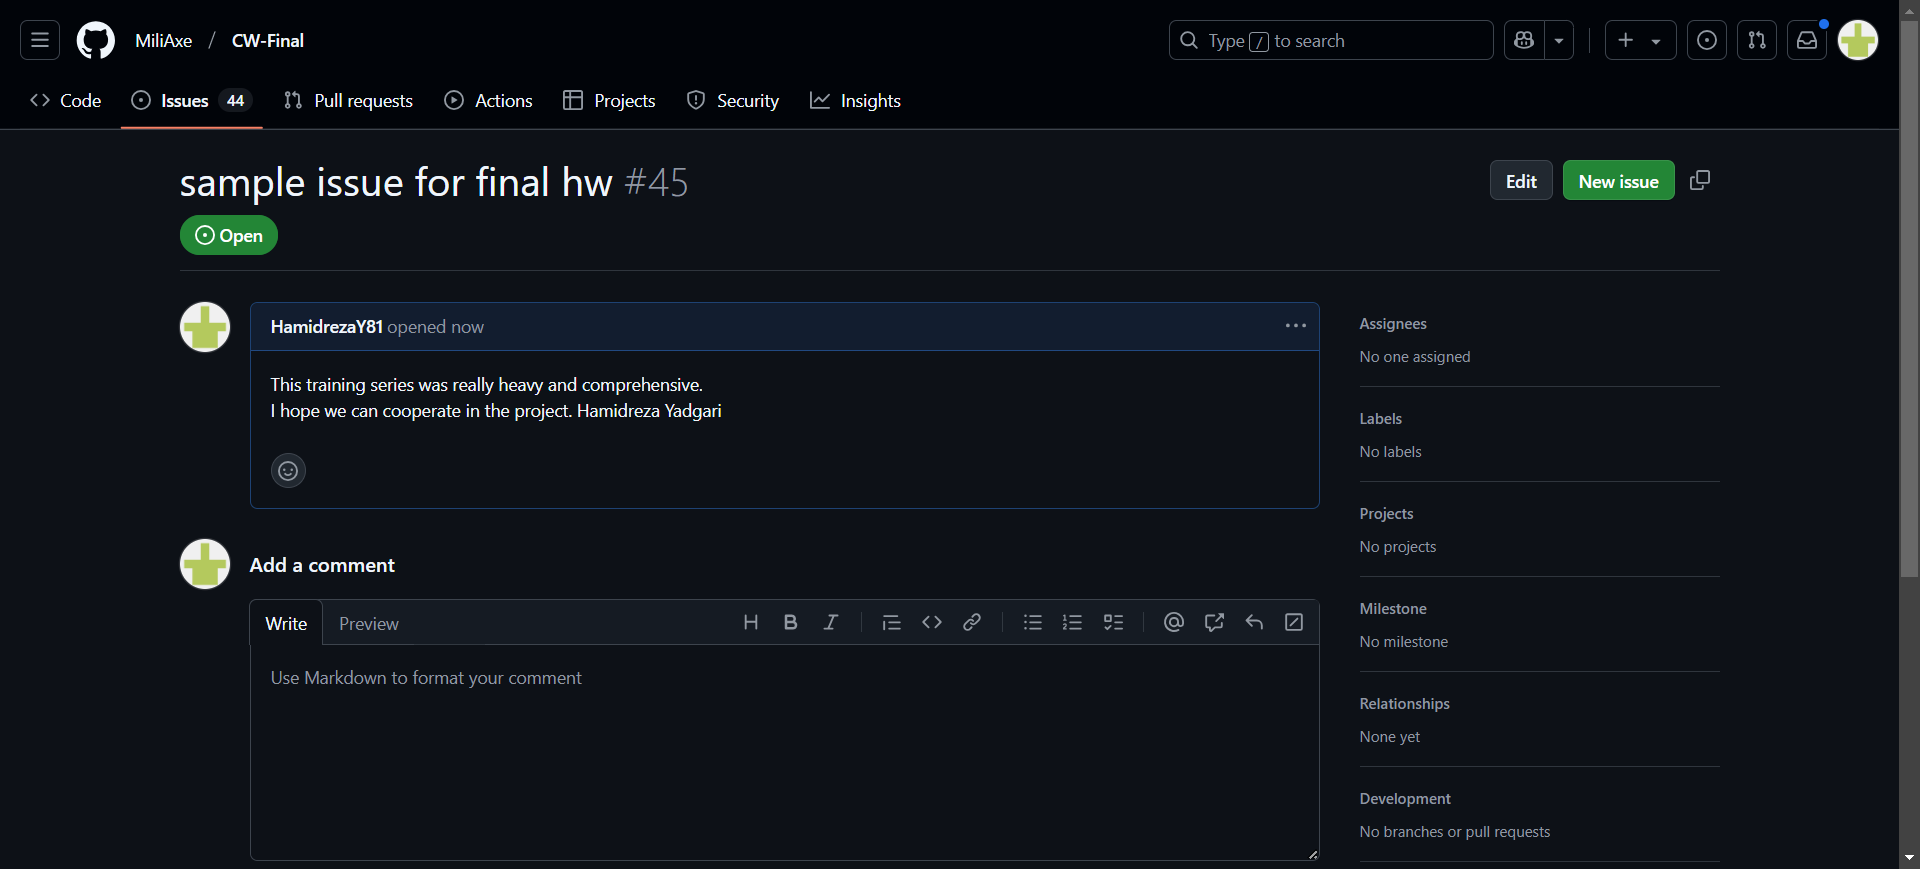
\includegraphics[width=0.8\textwidth]{hi.png}
            \caption{GitHub Issue}
        \end{figure}
        
    \subsection{FOSS contribution}
        In my opinion, it's absolutely right to be aware of the ins and outs of the tools we use. However, on the other hand, I feel that if everything is made transparent, the potential for earning could be reduced. Therefore, I'm uncertain and need to research more.
\end{document}
